\documentclass{article}
\usepackage{amsmath}
\usepackage{amssymb}
\usepackage{graphicx}
\graphicspath{ {./images/} }
\usepackage[utf8]{inputenc}
\usepackage{epigraph}
\title{HW Multi-factor Models}
\date{Nov 13rd 2018}
\author{Xia Xicheng}

\begin{document}
	\maketitle
\section{Performance Measurement}

\quad

Sharpe ratio measures the risk premium per unit of total risk;

Sortino Ratio measures the risk premium per unit of downside risk;

Jensen's Alpha measures the pricing error of CAPM;

Three-factor Alpha measures the pricing error of three-factor model.
\begin{figure}[h]
	\centering
	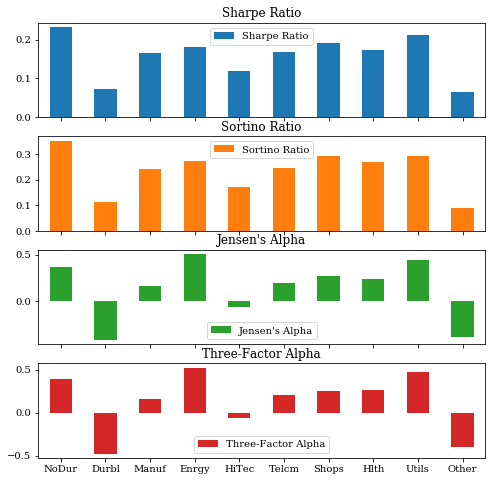
\includegraphics[width=9cm]{output_17_0.png}
\end{figure}

\section{Minimum-Variance Frontier Revisited}
\subsection{Calculate efficient frontier via scipy.optimize.minimize}
Before we apply Monte Carlo method, we firstly use scipy.optimize.minimize to find out the frontier portfolio weight.
\begin{figure}[h]
	\centering
	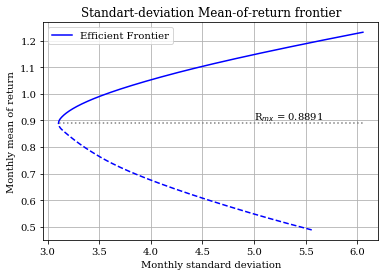
\includegraphics[width=9cm]{output_25_0.png}
\end{figure}

We can find that weight of optimal portfolio consists of a large proportion of extremely small values.
\begin{figure}[h]
	\centering
	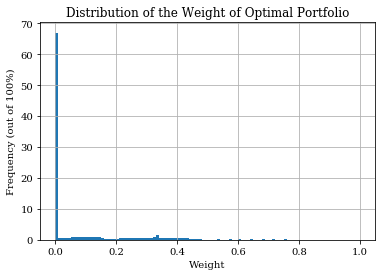
\includegraphics[width=9cm]{output_27_0.png}
\end{figure}

\subsection{Simulate efficient frontier via random weight generated by normal distribution}

Weight generated from normal distribution are not very likely to located on the optimal portfolio, because it doesn't countain enough proportion of extremely small weights.
\begin{figure}[h]
	\centering
	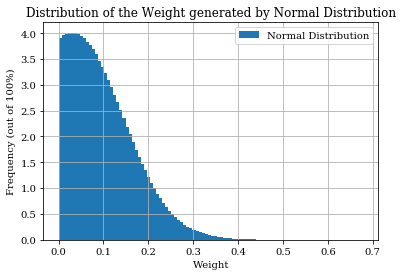
\includegraphics[width=9cm]{output_31_0.png}
\end{figure}

No surprise, the simulation fails to be perfectly located on the frontier.
\begin{figure}[h]
	\centering
	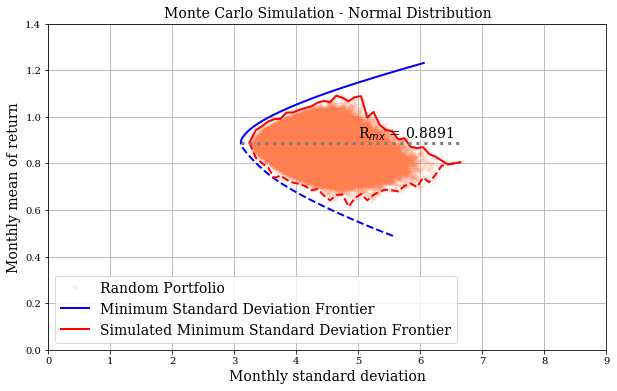
\includegraphics[width=9cm]{output_35_0.png}
\end{figure}

\newpage

\subsection{Simulate efficient frontier via random weight generated by reciprocal normal distribution}

Reciprocal of normal distribution can generate more extreme values than the original one.
\begin{figure}[h]
	\centering
	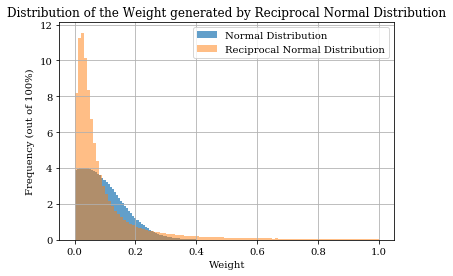
\includegraphics[width=9cm]{output_39_0.png}
\end{figure}

This time, the simulation is perfectly located on the frontier.
\begin{figure}[h]
	\centering
	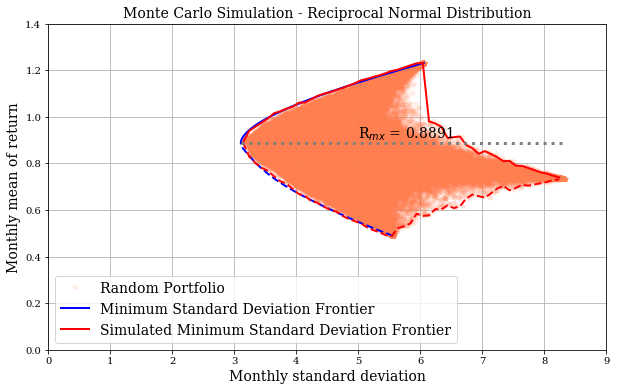
\includegraphics[width=9cm]{output_43_0.png}
\end{figure}

\section{Complementary Work : Uniform Distribution}

We can find out than reciprocal of uniform distribution can performs equally good as that of normal distribution.
\begin{figure}[h]
	\centering
	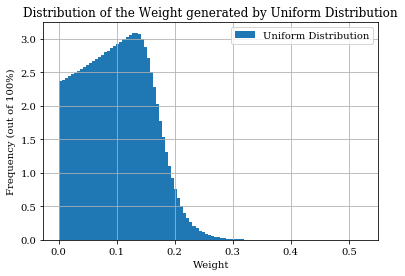
\includegraphics[width=9cm]{output_45_0.png}
\end{figure}
\begin{figure}[h]
	\centering
	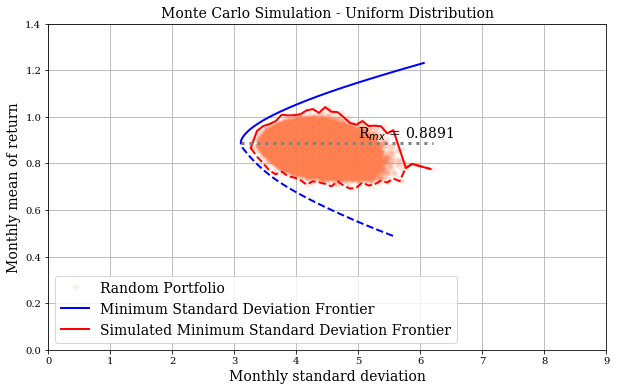
\includegraphics[width=9cm]{output_45_1.png}
\end{figure}
\begin{figure}[h]
	\centering
	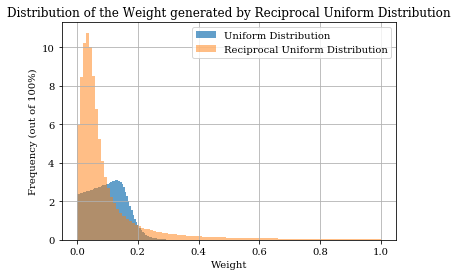
\includegraphics[width=9cm]{output_46_0.png}
\end{figure}
\begin{figure}[h]
	\centering
	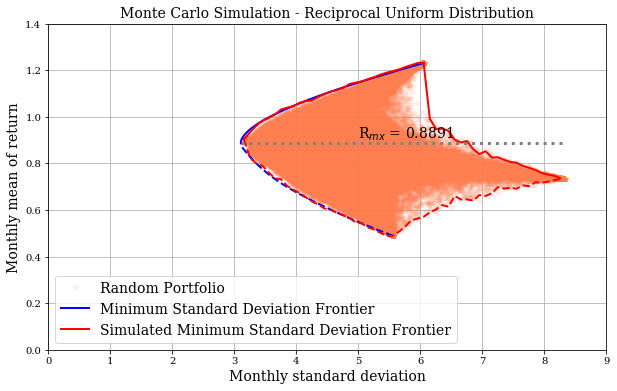
\includegraphics[width=9cm]{output_46_1.png}
\end{figure}
\end{document}